%-%-%-%-%-%-%-%-%-%-%-%-%-%-%-%-%-%-%-%-%-%-%-%-%-%
% EE531: laboratório de Eletrônica Básica I       %  
% Experimento 2: Diodos                           %
% Data:20/08/2010                                 %
% Unicamp,Campinas,São Paulo,Brasil               % 
% Grupo:                                          %
%       - Raquel Mayumi Kawamoto                  %
%       - Tiago Chedraoui Silva                   % 
%-%-%-%-%-%-%-%-%-%-%-%-%-%-%-%-%-%-%-%-%-%-%-%-%-%
%\documentclass[letter]{article}  % formato impressao IC
\documentclass[a4paper]{article} % formato impressao FEEC

%%% fontes %%%
\usepackage[T1]{fontenc}
\usepackage[brazil]{babel}    % dá suporte para os termos na língua portuguesa do Brasi
\usepackage[utf8]{inputenc}   % acentuação
\usepackage{ae,aecompl,aeguill}       % pdfs mais bonitos =)

%%% outros %%%
\usepackage{multirow}
\usepackage{textcomp}
\usepackage{color}       
\usepackage{indentfirst}      % retira padrao americano de paragrafos
\usepackage{multicol}   
\usepackage[linkbordercolor={1 1 1},urlcolor=black,colorlinks=true]{hyperref} % links
\usepackage{subfig}
\usepackage[letterpaper]{geometry}
\geometry{verbose,lmargin=3cm,rmargin=3cm}

% circuito eletrico
\usepackage{electComp}
\usetikzlibrary{decorations,decorations.pathmorphing,decorations.pathreplacing}
\usepackage{verbatim}
\usepackage{pstricks}
\usepackage{boxdims}


\date{Agosto 20, 2010}
% Capa estilizada %
\newcommand*{\titleTMB}{\begingroup \centering \settowidth{\unitlength}{\LARGE EE531} {\large\scshape EE531 - Turma S}\\[0.2\baselineskip] \rule{11.0cm}{1.6pt}\vspace*{-\baselineskip}\vspace*{2pt} \rule{11.0cm}{0.4pt}\\[\baselineskip] {\LARGE  Diodos}\\\vspace*{\baselineskip}  {\itshape Laboratório de Eletrônica Básica I - Segundo Semestre de 2010}\\ \rule{11.0cm}{0.4pt}\vspace*{-\baselineskip}\vspace{3.2pt} \rule{11.0cm}{1.6pt}\\[\baselineskip] {\large\scshape Professor: José Cândido Silveira Santos Filho}\par \vfill {\normalsize   \scshape 
    \begin{center} 
      \begin{tabular}{  l  l  p{5cm} } 
 	Daniel Lins Mattos & RA: 059915\\
        Raquel Mayumi Kawamoto & RA: 086003\\
        Tiago Chedraoui Silva  & RA: 082941\\
      \end{tabular} \end{center}
    \itshape 10 de setembro de 2010    }\\[\baselineskip] \vspace{3.2pt} \endgroup}


\begin{document}
\titleTMB 
\newpage

\vspace{3mm}
\begin{figure}[h]
\centerline{\input circ1.tex}
\caption{Circuito para caracterização V versus I do diodo \label{tab:circ}}
\end{figure}

\vspace{3mm}
\begin{figure}[h]
\centerline{\input circ2.tex}
\caption{Circuito retificador de meia onda \label{tab:circ}}
\end{figure}

\vspace{3mm}
\begin{figure}[h]
\centerline{\input circ3.tex}
\caption{Circuito retificador de onda completa  \label{tab:circ}}
\end{figure}


\newpage
\vspace{3mm}
\begin{figure}[h]
\centerline{\input circ4.tex}
\caption{Duplicador de tensão \label{tab:circ}}
\end{figure}



\begin{figure}[h!]
\begin{centering}
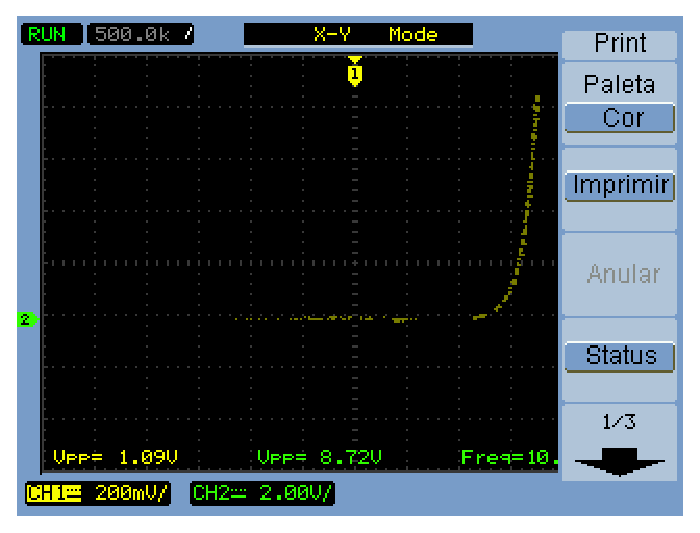
\includegraphics[scale=0.7]{Imagens/3.1/q1} \caption{Curva característica V versus I do diodo \label{fig:q1-curva}}
\par\end{centering}
\end{figure}


\begin{figure}[h!]
\begin{centering}
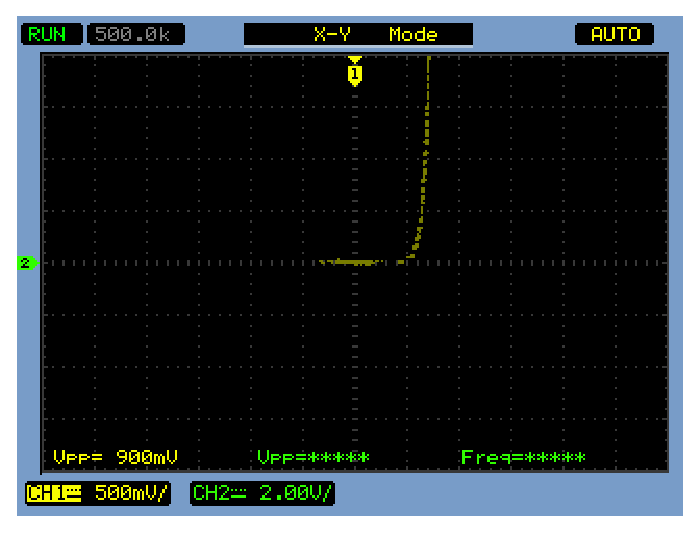
\includegraphics[scale=0.7]{Imagens/3.1/NewFile0} \caption{Curva característica V versus I do diodo  \label{fig:q1-curva2}}
\par\end{centering}
\end{figure}


\begin{figure}[h!]
\begin{centering}
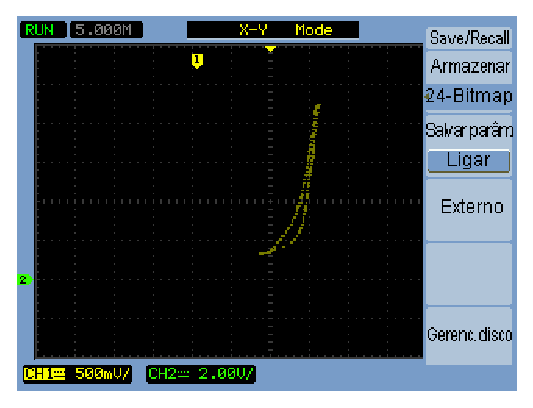
\includegraphics[scale=1.0]{Imagens/3.1.opcional/opcio} \caption{Curva de histerese \label{fig:q1-his}}
\par\end{centering}
\end{figure}

\newpage
\begin{figure}[h!]
\begin{centering}
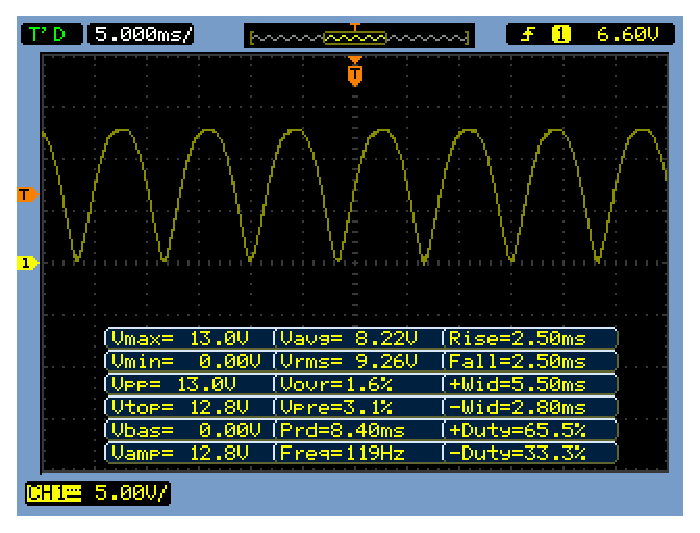
\includegraphics[scale=0.7]{Imagens/3.3.1onda_completa/3} \caption{Medida da tensão no nó 3 \label{fig:q2-no3}}
\par\end{centering}
\end{figure}



\begin{figure}[h!]
\begin{centering}
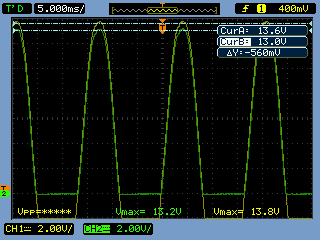
\includegraphics[scale=0.7]{Imagens/3.3.1onda_completa/31} \caption{Medida da tensão diferencial entre os nós 2 e 3 \label{fig:Fig-45}}
\par\end{centering}
\end{figure}


\begin{figure}[h!]
\begin{centering}
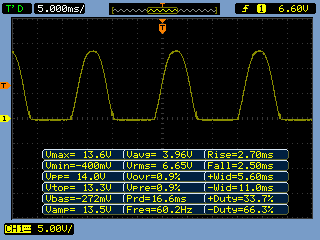
\includegraphics[scale=0.7]{Imagens/3.3.1onda_completa/no1} \caption{Medida da tensão no nó 1 \label{fig:q2-no1}}
\par\end{centering}
\end{figure}

\newpage
\begin{figure}[h!]
\begin{centering}
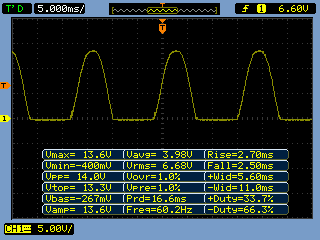
\includegraphics[scale=0.7]{Imagens/3.3.1onda_completa/no2} \caption{Medida da tensão no nó 2  \label{fig:q2-no2}}
\par\end{centering}
\end{figure}


\begin{figure}[h!]
\begin{centering}
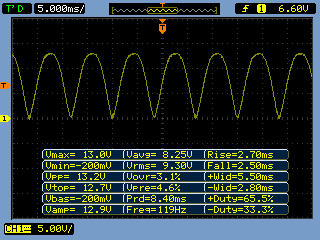
\includegraphics[scale=0.7]{Imagens/3.3.1onda_completa/no3} \caption{Medida da tensão diferencial entre os nós 2 e 3 \label{fig:Fig-45}}
\par\end{centering}
\end{figure}


\begin{figure}[h!]
\begin{centering}
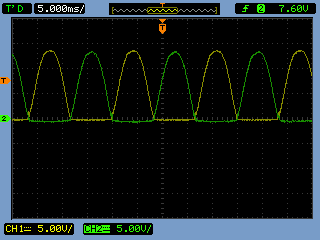
\includegraphics[scale=0.7]{Imagens/3.3.1onda_completa/no12} \caption{Medida da tensão nos nós 1 e 2 \label{fig:Fig-45}}
\par\end{centering}
\end{figure}


\begin{figure}[h!]
\begin{centering}
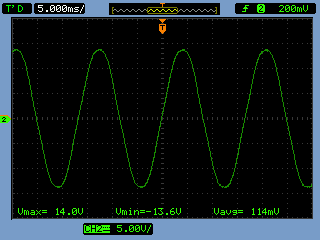
\includegraphics[scale=0.7]{Imagens/3.3.1onda_completa/p1q3} \caption{Medida da tensão diferencial entre os nós 2 e 3 \label{fig:Fig-45}}
\par\end{centering}
\end{figure}



\newpage
\begin{figure}[h!]
\begin{centering}
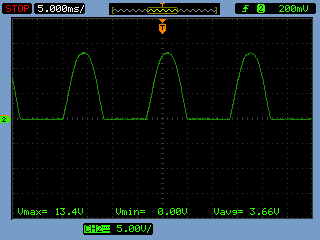
\includegraphics[scale=0.7]{Imagens/3.3.1onda_completa/p2q3} \caption{Medida da tensão diferencial entre os nós 2 e 3 \label{fig:Fig-45}}
\par\end{centering}
\end{figure}

\begin{figure}[h!]
\begin{centering}
\includegraphics[scale=0.7]{Imagens/3.3.1ret_meia_onda/311} \caption{Medida da tensão diferencial entre os nós 2 e 3 \label{fig:Fig-45}}
\par\end{centering}
\end{figure}

\begin{figure}[h!]
\begin{centering}
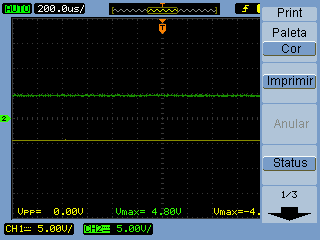
\includegraphics[scale=0.7]{Imagens/3.4duplicador_tensao/423} \caption{Medida da tensão diferencial entre os nós 2 e 3 \label{fig:Fig-45}}
\par\end{centering}
\end{figure}


\newpage
\begin{figure}[h!]
\begin{centering}
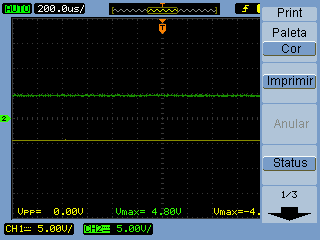
\includegraphics[scale=0.7]{Imagens/3.4duplicador_tensao/423} \caption{Tensão de saída nos nós 1 e 2 \label{fig:q4-no12}}
\par\end{centering}
\end{figure}


\begin{figure}[h!]
\begin{centering}
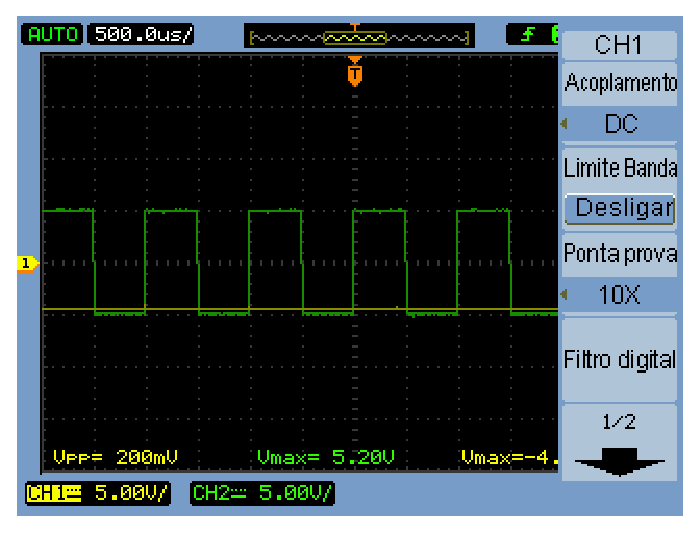
\includegraphics[scale=0.7]{Imagens/3.4duplicador_tensao/444} \caption{Análise do sinal de saída no nó x \label{fig:q4-no}}
\par\end{centering}
\end{figure}


\begin{figure}[h!]
\begin{centering}
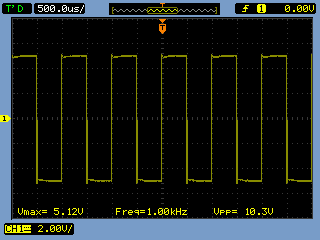
\includegraphics[scale=0.7]{Imagens/3.4duplicador_tensao/Vin} \caption{Onda de entrada do circuito\label{fig:q4-vin}}
\par\end{centering}
\end{figure}



\begin{figure}[h!]
\begin{centering}
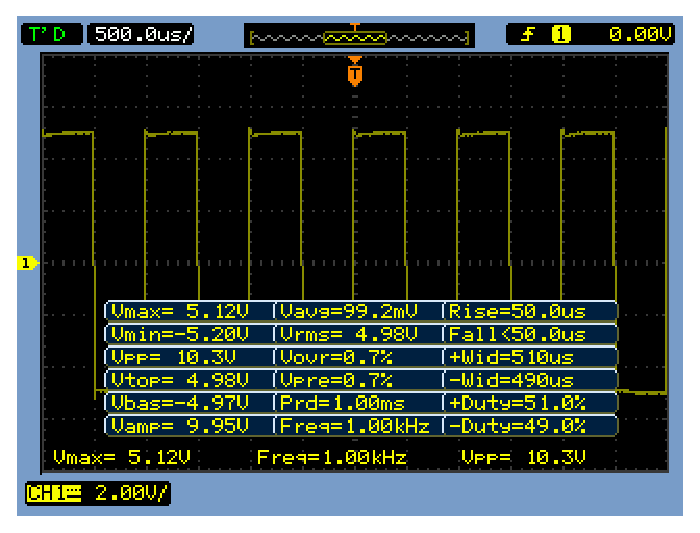
\includegraphics[scale=0.7]{Imagens/3.4duplicador_tensao/Vinmedidas} \caption{Medidas da onda de entrada do circuito \label{fig:q4-vindata}}
\par\end{centering}
\end{figure}


\newpage
\begin{figure}[h!]
\begin{centering}
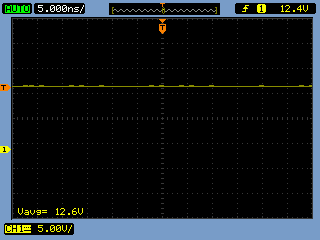
\includegraphics[scale=0.7]{Imagens/3.3.4capacitor_paralelo/3cao1} \caption{Característica onda após a inserção de capacitor em paralelo \label{fig:Fig-45}}
\par\end{centering}
\end{figure}


\begin{figure}[h!]
\begin{centering}
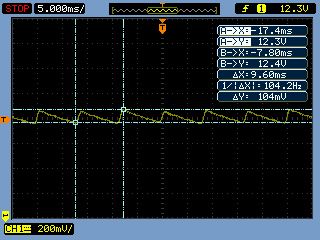
\includegraphics[scale=0.7]{Imagens/3.3.4capacitor_paralelo/3cap} \caption{Aproximação da imagem da onda após a inserção de capacitor em paralelo \label{fig:q2-cap}}
\par\end{centering}
\end{figure}


\end{document}
